% This file contains the text portion of the System Overview portion of the project charter

% 7 SYSTEM OVERVIEW
It is assumed that the drone will be equipped with a single-board computer in the diagram below. Using a single-board computer, the drone would be able to process the tasks it is required to carry out for each showcase by executing them through the single-board computer. It is still unknown whether the computation part of the project will be allowed to be performed wirelessly (i.e. without the need for an onboard computer to control the drone) by the team. Once a decision has been made, a new version of this document will be prepared.

It is expected that a flight controller will be mounted on the drone in order to control the motors' speeds, therefore allowing horizontal and vertical movement in the drone to take place. It will be necessary to run Mission Planner on a computer (either onboard or via a wireless connection) in order for it to function. With the help of Mission Planner, drone movements can be mapped for the drone so it can be controlled as needed. With Mission Planner, autonomous vehicles can communicate with a ground station via an interface which can be accessed from most Windows operating systems. As a result of using Mission Planner, the team will have the option of creating their own autonomous flight paths. Further, the computer will run a program that has the capability of identifying ArUco markers as well as functioning as a link between the computer and the flight controller.

For aiming at the ace combat sensors that are located on all hostile ground vehicles, there needs to be a laser attached close to the camera to increase accuracy. There are two choices available to the camera once it detects an ArUco marker. The camera can either turn and aim at the enemy vehicle or move to a position where the drone could use its laser to shoot moving ground vehicles.

There will be a dedicated flight controller that will be connected to GPS and RTK systems. It is expected that the drone motors will be connected to electronic speed controllers, which will in turn be connected to the dedicated flight controller.

To power all of the components of the drone while it is in flight, the drone will need to be equipped with a battery. There is no doubt that batteries can add a lot of weight to a drone, so this is also something that should be considered when deciding which batteries to use. Battery size and location should also be considered in order to ensure that the camera or laser is not interfered with or blocked by the battery in any way.

\begin{figure}[h!]
    \centering
    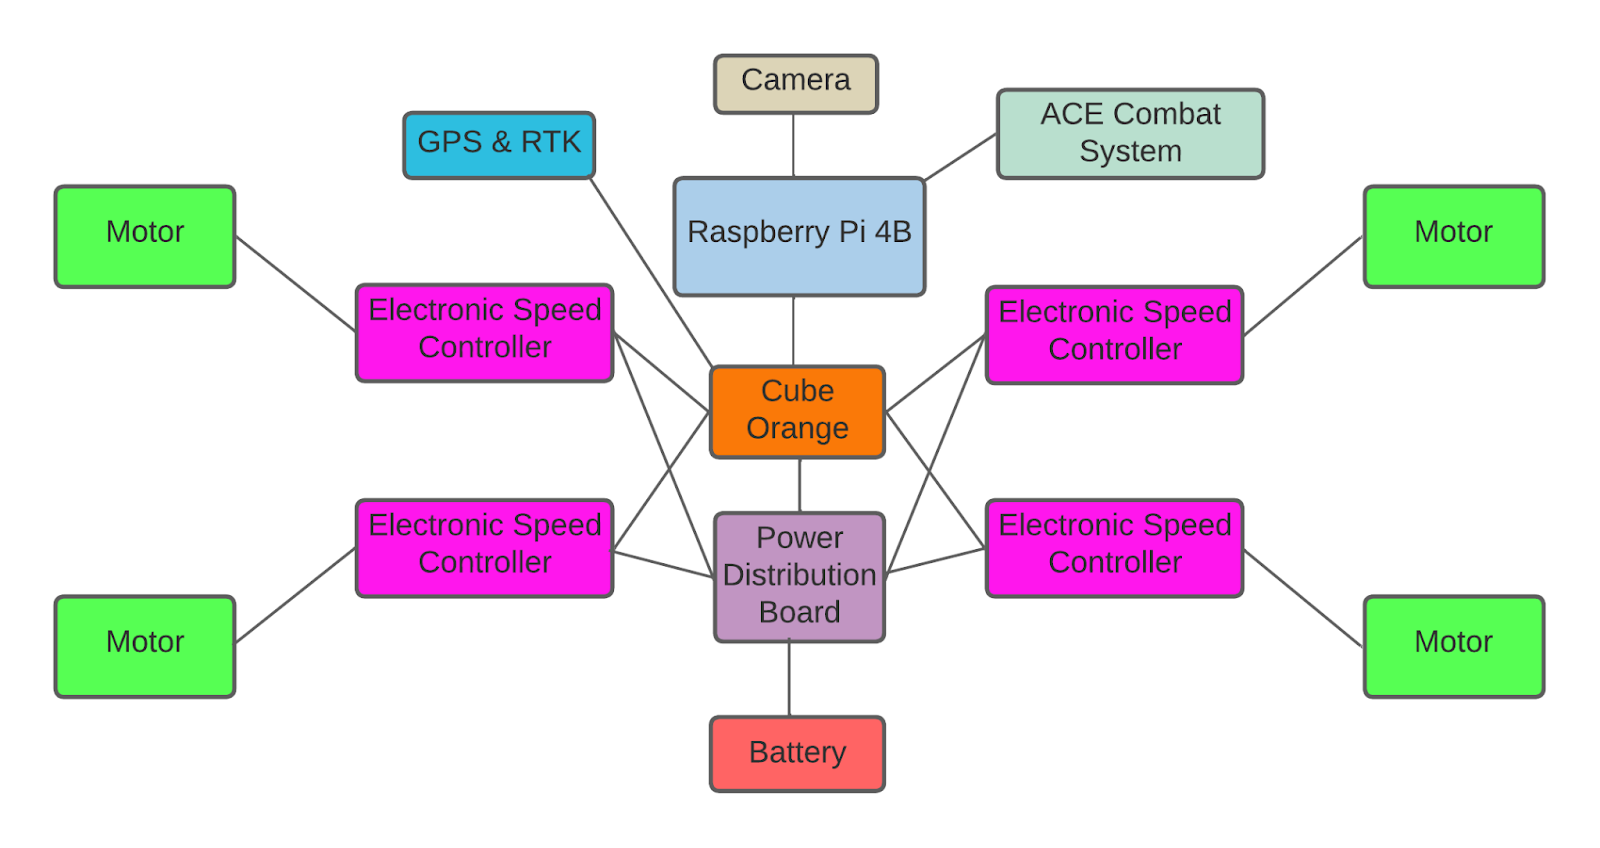
\includegraphics[width=1\textwidth]{images/system_overview.png}
    \caption{Diagram of the System Overview}
\end{figure}
